%%%%%%%%%%%%%%%%%%%%%%%%%%%%%%%%%%%%%%%%%
% Friggeri Resume/CV
% XeLaTeX Template
% Version 1.0 (5/5/13)
%
% This template has been downloaded from:
% http://www.LaTeXTemplates.com
%
% Original author:
% Adrien Friggeri (adrien@friggeri.net)
% https://github.com/afriggeri/CV
%
% License:
% CC BY-NC-SA 3.0 (http://creativecommons.org/licenses/by-nc-sa/3.0/)
%
% Important notes:
% This template needs to be compiled with XeLaTeX and the bibliography, if used,
% needs to be compiled with biber rather than bibtex.
%
%%%%%%%%%%%%%%%%%%%%%%%%%%%%%%%%%%%%%%%%%

\documentclass[a4paper,latin]{friggeri-cv} % Add 'print' as an option into the square bracket to remove colors from this template for printing
\hypersetup{
pdftitle={Bewerbungsunterlagen von Sascha Manns}, %%
pdfauthor={Sascha Manns}, %%
pdfsubject={Bewerbungsunterlagen}, %%
pdfcreator={XeLaTEX and Biber with hyperref-package.},
pdfproducer={Sascha Manns, Mayen}, %%
pdfkeywords={Manns, Mayen, Bewerbung, IT, Community, Linux, Programmierer, Dispatcher, Buchautor} %%
}
\usepackage{pdfpages}
\usepackage{graphicx}
\usepackage{xltxtra}
%\usepackage{rotating}

\addbibresource{../Appendix/Bibliography/bibliography1.bib} % Specify the bibliography file to include publications
\def\firstname{Sascha}
\def\familyname{Manns}
\def\mystreet{Maifeldstraße 10}
\def\mycity{56727 Mayen}
\def\myphone{+49-2651-40~14~045}
\def\myemail{Sascha.Manns@bdvb.de}

\begin{document}
%\includepdf{../Anschreiben/bwanschreiben} %bei Bedarf uncommenten
\includepdf{../Cover/Cover}

\header{Sascha}{Manns}{Autor Geschäftsprozessdokumentation} % Your name and current job title/field

%----------------------------------------------------------------------------------------
%	SIDEBAR SECTION
%----------------------------------------------------------------------------------------

\begin{aside} % In the aside, each new line forces a line break
\section{Kontakt}
Maifeldstraße 10
56727 Mayen
Germany
~
+49 (2651) 40 14 045
+49 (1573) 924 2730
~
\href{mailto:Sascha.Manns@directbox.com}{Sascha.Manns@directbox.com}
\href{http://saigkill.github.io}{saigkill.github.io}
\href{https://www.xing.com/profile/Sascha_Manns2}{xi://Sascha.Manns2}
\href{http://de.linkedin.com/in/saigkill}{li://saigkill} 
\section{Fremdsprachen}
Deutsch Muttersprache
Englisch
\section{Programming}
{Shell (Bash)}
{JavaScript}
{CSS \& HTML5}
{Ruby}
\end{aside}

%----------------------------------------------------------------------------------------
%	WORK EXPERIENCE SECTION
%----------------------------------------------------------------------------------------

\section{Berufserfahrung}

\begin{entrylist}
%------------------------------------------------
\entry{09/2014--08/2015}
{XCOM AG}
{Andernach}
{\emph{Autor Geschäftsprozessdokumentation} \\
	Detailierte Aufgaben:
	\begin{itemize}
		\item Autor Geschäftsprozessdokumentation (Software  \& Bankwesen)
		\item Artikelerstellung und Pflege internes Wiki
		\item Produktion Präsentationen für Mandanten und interne Schulungen
		\item Modellierung von Geschäftsprozessen nach BPMN
	\end{itemize}
}
%------------------------------------------------
\entry
{02/2014--05/2014}
{Hays Temp GmbH}
{Mannheim}
{\emph{IT-Supporter} \\
Detailierte Aufgaben bei ITSCare Neuwied (ZBV):
\begin{itemize}
\item Kundenpflege via Telefon und Email
\item Dispatching und Teamcontroling
\item AmSys/IDM (AOK Krankenkassen)
\item Eröffnung, Entsperrung oder Löschung von Benutzerkonten
\item Passwort- und Rechtevergaben
\item SLA-konforme Bearbeitung von eingehenden Störungen (betreffend Benutzerverwaltung) im Rahmen des Incident-Managements
\item Pflege von Logon-Prozeduren
\item Annahme, Erfassung und Bearbeitung eingehender Benutzeranträge
\item Benutzerkontenverwaltung im Active Directory
\end{itemize}
}
%------------------------------------------------
\entry
{11/2012--10/2013}
{Lulu Press Inc.}
{Homeoffice}
{\emph{Buchautor \& Herausgeber}\\
Detailierte Aufgaben:
\begin{itemize}
\item Recherche
\item Schreiben des Handbuchs
\item Einführung des Lektorenteams in das Projekt
\item Einführung einer Google Code-In Studentin in den Textsatz (Teilnahme als Mentor)
\item Satz \& Layout (\LaTeX{} und DocBook/XSL-FO)
\end{itemize}
}
%------------------------------------------------
\entry
{08/2012--06/2013}
{open-slx GmbH}
{Homeoffice}
{\emph{Community \& Support Agent} \\
Detailierte Aufgaben:
\begin{itemize}
\item Level 1 \& 2 Support via Telefon und Email
\item Testen von Software
\item Webseitenbetreuung \& Social Media
\item Dokumentation
\item Pflege der Supportdatenbank
\item Öffentlichkeitsarbeit
\item Community Management
\item Informationsaustausch mit Produktmanagement
\end{itemize}
}
%------------------------------------------------
\entry
{08/2011--07/2012}
{open-slx GmbH}
{Homeoffice}
{\emph{Langzeitpraktikum} \\
Detailierte Aufgaben:
\begin{itemize}
\item Produktvorbereitung
\item Produkttesting
\item Verfassung des Handbuches
\item Öffentlichkeitsarbeit \& Social Media
\end{itemize}
}
\end{entrylist}
\begin{entrylist}
%------------------------------------------------
\entry
{08/2010--08/2011}
{open-slx GmbH}
{Homeoffice}
{\emph{Freiwillige Mitarbeit}\\
Detailierte Aufgaben:
\begin{itemize}
\item Projektleitung deutsches openSUSE Wiki. Migration des Wikis zu neuer Struktur
\item openSUSE Weekly News
\item Paketverwaltung einiger RPM-Pakete
\item openSUSE Membership Application Team
\item Import der Wiki-Unterlagen in open-slx Wikis 
\end{itemize}
}
%------------------------------------------------
\entry
{08/2011--jetzt}
{openSUSE Linux Projekt}
{Homeoffice}
{\emph{Paketbetreuer}\\
Detailierte Aufgaben:
\begin{itemize}
\item Beschaffung, Aktualisierung des Sourcecodes im Buildservice
\item Compiling und Packaging neuer Binärpakete
\item Verteilung via Buildservice
\end{itemize}
}
%------------------------------------------------
\entry
{07/2007--08/2011}
{openSUSE Linux Projekt}
{Homeoffice}
{\emph{Teamleiter}\\
Tätigkeiten:
\begin{itemize}
\item Leiter des openSUSE Newsletters und Publikationen in bis zu 12 Sprachen
\item openSUSE Medical Project (Subprojektgründer)
\item Mitglied des openSUSE Marketing Teams
\item Mitglied des openSUSE Feature Screening Teams
\end{itemize}
}
%-----------------------------------------------
\entry
{07/2000--06/2007}
{WTG}
{Selters/Ts.}
{\emph{Ersatzdienst zum Zivildienst}\\
Detailierte Aufgaben:
\begin{itemize}
\item Anlernen zum Maler \& Bodenleger
\item Projektleitung in der Bodenverlegung
\item Inventurleitung
\item Key-User
\end{itemize}
}
\end{entrylist}
\begin{entrylist}
%------------------------------------------------
\entry
{08/1998--07/2000}
{Auto Deschner GmbH}
 {Mendig}
{\emph{Kaufmann im Einzelhandel}\\
Detailierte Aufgaben:
\begin{itemize}
\item Einkauf \& Warenannahme \& Kontrolle
\item Bestandsbuchungen der Waren
\item Kundenbetreuung
\item Rechnungserstellung
\item Projektplanung
\end{itemize}
}
\end{entrylist}

\section{Berufsausbildung}
\begin{entrylist}
%------------------------------------------------
\entry
{08/1995--08/1998}
{Auto Deschner GmbH}
{Mendig}
{\emph{Ausbildung zum Kaufmann im Einzelhandel}\\
allgemeine kaufm. Tätigkeiten.
}
%------------------------------------------------
\end{entrylist}

%----------------------------------------------------------------------------------------
%	EDUCATION SECTION
%----------------------------------------------------------------------------------------

\section{Weiterbildung \& Zertifikate}

\begin{entrylist}
%------------------------------------------------
\entry
{02/2013--jetzt}
{Studium (berufsbegl.): Staatlich geprüfter Betriebswirt}
{ILS, Hamburg}
{Schwerpunkt Wirtschaftsinformatik}
%------------------------------------------------
\entry
{12/2013}
{Web Engeneering 1}
{Technische Hochschule Mittelhessen}
{\emph{MOOC}}
%------------------------------------------------
\entry
{06/2013}
{Kompetenzpass für Ökonomen}
{BV Deutscher Volks- und Betriebswirte}
{Düsseldorf}
%------------------------------------------------
\entry
{04/2013}
{Onlinequalifizierung: Schlüsselkompetenzen kompakt}
{Career Webinars}
{Web}
%-----------------------------------------------
\end{entrylist}

\section{Weiterbildung online: Microsoft Virtual Academy}
\begin{itemize}
\item Moderne Softwareentwicklung
\end{itemize}

%----------------------------------------------------------------------------------------
%	EHRENAMTLICHE TÄTIGKEITEN
%----------------------------------------------------------------------------------------
\newpage 
\section{Ehrenamtliche Tätigkeiten}
\begin{entrylist}
%--------------------------------------------
\entry
{2013-jetzt}
{mUXCamp 2014}
{mUXCamp, Worms}
{Planungsteam für nächstes Camp. (Mitveranstalter: \\FG Wirtschaftsinformatik des BDVB)}
%--------------------------------------------
\entry
{2013--jetzt}
{BV Deutscher Volks- und Betriebswirte}
{FG Wirtschaftsinformatik}
{Mitarbeit in verschiedenen Projekten}
%----------------------------------------------
\entry
{2013--jetzt}
{Gesellschaft für Informatik}
{FG Wirtschaftsinformatik}
{Mitarbeit in verschiedenen Projekten}
%---------------------------------------------
\entry
{2013--jetzt}
{Forum Informatiker für Frieden und gesellschaftliche Verantwortung}
{}
{}
%--------------------------------------------
\entry
{2010--2011}
{Piratenpartei Deutschland}
{Bundespressestelle}
{}
%--------------------------------------------
\entry
{2008--jetzt}
{openSUSE Linux Project}
{Membership Application Team/RPM Packaging}
{Mitgliederverwaltung \& Paketverwaltung}
%--------------------------------------------
\end{entrylist}

%----------------------------------------------------------------------------------------
% COMPUTER SKILLS
% ---------------------------------------------------------------------------------------

\section{IT-Kenntnisse}

\begin{itemize}
\item OS: Linux/Unix, Windows 3.11--8.1
\item ERP/CRM: ADP Opel Verkäuferarbeitsplatz, oscare (SAP Lösung für Gesundheitsbranche)
\item Packaging: RPM, Compiling/Testing/Publishing, git, svn
\item Textsatz: \LaTeX, XML/DocBook 4.5 \& XSL-FO
\item Translations: FreeMedForms, KVirusTotal (Übersetzung EN $\triangleright$ DE)
\item Administration: Linux/Unix
\item Webservices: Apache2, Joomla, Owncloud, Wordpress, Hosting, Mediawiki, SVN-Server, MySQL, Cloudcontrol Appliances
\item Multimedia: Pod- \& Screencastproduktionen, Videoschnitt
\item Office: MS/Libre-Office, Projektmanagement-Software, Lexware
\item Produktgestaltung: Handbucherstellung, Supportdatenbank, Webpräsentation
\item Wissensmanagement: MS Sharepoint, Business Wiki, Business Social Networks
\item Erweiterte Kenntnisse: Warenwirtschaftssysteme, Auftragsmanagementsysteme, OTRS, Mantis, Amsys, IDM, Oxygen XML-Editor
\item IDEs: Visual Studio, RubyMine, Webstorm, IntelliJ
\end{itemize}

%----------------------------------------------------------------------------------------
%	COMMUNICATION SKILLS SECTION
%----------------------------------------------------------------------------------------

\section{Kommunikation}

\begin{entrylist}
%------------------------------------------------
\entry
{2013}
{mUXCamp Worms}
{Standbetreuung}
{Vertretung der FG Wirtschaftsinformatik des BDVB}
%------------------------------------------------
\entry
{2010}
{openSUSE Conference}
{Vortrag}
{Vortrag über den aktuellen Stand der Weekly News und die Planungen der Zukunft}
%------------------------------------------------
\entry
{2010}
{openSUSE Conference}
{Vortrag}
{Vortrag über Open Source im Alltag}
%------------------------------------------------
\end{entrylist}

%----------------------------------------------------------------------------------------
%	INTERESTS SECTION
%----------------------------------------------------------------------------------------

\section{Interessen}

\textbf{professional:} Büroorganisation, Software, Webdesign, Web-App-Erstellung, Marketing \\ 
\textbf{personal:} Literatur (IT/Wirtschaft/Philosophie), Wandern, Bücher schreiben, Netzwerken (Real Life)

%----------------------------------------------------------------------------------------
%	PUBLICATIONS SECTION
%----------------------------------------------------------------------------------------
\newpage 
\section{Publikationen}

\printbibsection{article}{Artikel} % Print all articles from the bibliography

\printbibsection{book}{Bücher} % Print all books from the bibliography

\begin{refsection} % This is a custom heading for those references marked as "inproceedings" but not containing "keyword=france"
\nocite{*}
\printbibliography[sorting=chronological, type=inproceedings, title={international peer-reviewed conferences/proceedings}, notkeyword={france}, heading=subbibliography]
\end{refsection}

\begin{refsection} % This is a custom heading for those references marked as "inproceedings" and containing "keyword=france"
\nocite{*}
\printbibliography[sorting=chronological, type=inproceedings, title={local peer-reviewed conferences/proceedings}, keyword={france}, heading=subbibliography]
\end{refsection}

\printbibsection{misc}{other publications} % Print all miscellaneous entries from the bibliography

\printbibsection{report}{research reports} % Print all research reports from the bibliography

%----------------------------------------------------------------------------------------

\begin{center}

\includegraphics[scale=0.7]{../Pictures/signatur.png} \\
\begin{tabular}{@{}l@{}}
\\ $\frac{}{\strut\textnormal{Sascha Manns, Mayen den \today}}$
\end{tabular}
\end{center}

%\section{Anhang}
%---------------------------------------------------------------------------
% Include PDF
\begin{figure}  
  
\includegraphics[page=1,scale=0.7,angle=180]{../Appendix/Employers_Reference/hays.pdf}
\end{figure}

\includepdf{../Appendix/Study/foo}
%
\includepdf{../Anlagen/Arbeitszeugnisse/hays}

\includepdf{../Appendix/Certificates/thm-webeng1}
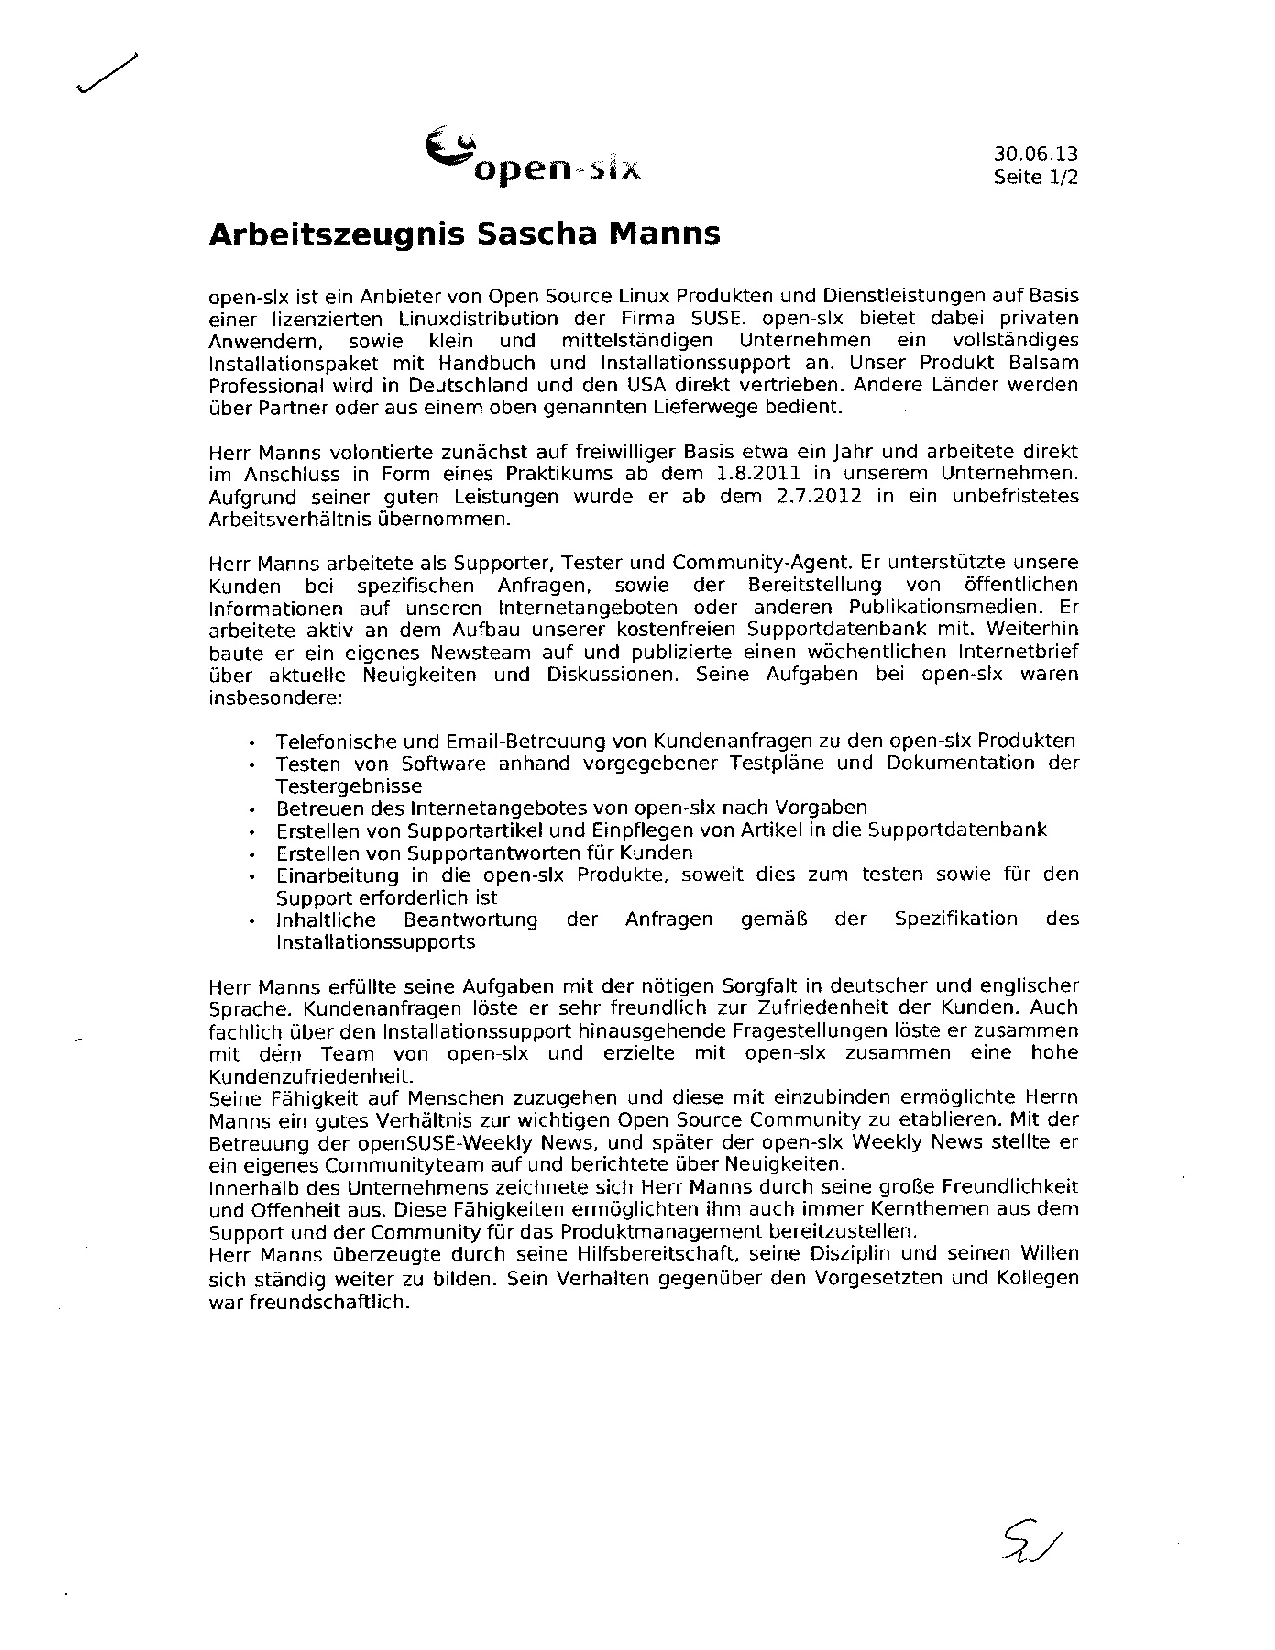
\includepdf{../Appendix/Employers_Reference/openslx}

\includepdf{../Appendix/Employers_Reference/openslx1}

\includepdf{../Appendix/Certificates/kompetenzpass12013}

\includepdf{../Appendix/Certificates/Zertifikat_Sascha_Manns1}

\includepdf{../Appendix/Employers_Reference/wtg}

\includepdf{../Appendix/First_References/ihk}

\end{document}
